\documentclass{aa}
\usepackage[varg]{txfonts}
\usepackage{color}
\usepackage{graphicx}
\usepackage{subfig}    %% For generating a grid of figures.
%% \newsavebox\mybox   %% For generating figure captions which wrap at figure 
%% edges.
%% \newlength\myboxlen
%% \newcommand{\figcap}[2]
%% {%
%%   \sbox\mybox{#1}
%%   \settowidth{\myboxlen}{\usebox{\mybox}}
%%   \centering
%%   \usebox\mybox
%%   \hskip \textwidth
%%   \parbox{\myboxlen}{#2}
%% }

\usepackage{bm}
\bibpunct{(}{)}{;}{a}{}{,} % to follow the A&A style
\begin{document}

\title{Design and Commissioning of the AARTFAAC all-sky monitor}

\author{Peeyush Prasad  \inst{1,2} \and Folkert Huizinga \inst{1} \and John Romein \inst{2}
\and Daniel van der Schuur \inst{2} \and Ralph  Wijers  \inst{1}}
 \institute{Universiteit  van
  Amsterdam \and ASTRON, The Netherlands Foundation for Radio Astronomy}

\date{Received <date> / Accepted <date>}

%% Structured abstract
\abstract{The  Amsterdam-ASTRON Radio  Transients Facility  And Analysis  Center
  (AARTFAAC)  array is  a  sensitive,  all-sky radio  imager  based  on the  Low
  Frequency Array (LOFAR). It generates images of the low frequency radio sky in
  near real-time with spatial resolution of  10s of arcmin, MHz bandwidths and a
  time cadence  of a few  seconds. The image  timeseries are then  monitored for
  short and  bright radio transients. On  detection of a transient,  low latency
  triggers  will  be  generated  for   LOFAR,  which  can  carry  out  follow-up
  observations.   In  this   paper,  we  describe  the   implementation  of  the
  instrumentation, and its capabilities.}

  \keywords{Radio Interferometry - Imaging - Radio Transients - Correlators}

\maketitle

\section{\label{sec:Introduction}Introduction}


<TODO: Paragraph about  transient sources, some stuff about  spectral indices of
coherent emission and  expected class of sources, at what  brightness levels can
we expect to see things (take from Lazio LWA paper).>

<TODO: Paragraph  summarizing the  current state of  knowledge of  low frequency
transients: Stewart NCP transient, other  searches at low freq. Conclusion: Need
for more monitoring.>


The AARTFAAC radio  transient monitor is a  leading effort among a  group of new
radio telescopes aiming for detection of  bursts of radio emission by continuous
monitoring of the low radio frequency sky.  Such telescopes are characterized by
having  moderate   resolution  and  sensitivity  as   compared  to  contemporary
telescopes, but  with extremely wide  fields of  view (typically all  sky), high
availabilities and autonomous calibration  and imaging.  The latter requirements
make their implementations challenging. The antenna elements used to achieve the
wide  fields  of view  are  typically  dipoles,  however, their  low  individual
sensitivities requires  an order of magnitude  larger number of elements  in the
array.   Bringing the  resulting  large  number of  data  streams  to a  central
location,  as well  as their  correlation fora  carrying out  aperture synthesis
imaging thus  poses a significant I/O  and compute challenge. Further,  the wide
fields  of view  at  the sensitivities  of operation  also  result in  direction
dependent effects on  the incoming signals, mostly due to  the ionosphere. These
pose a  challenge to calibration, especially  when carried out in  an autonomous
manner.  

In this  paper, we describe  the implementation  of the instrumentation  for the
AARTFAAC  array,  and the  commissioning  of  its various  subsystems.   Section
\ref{sec:aartfaac_array} describes the array and the receiving antenna elements,
its  relationship  with LOFAR,  and  introduces  the  full architecture  of  the
instrument.    Section   \ref{sec:station_hardware}   describes   the   hardware
implementation in  the field which  allows creating a  data path in  parallel to
LOFAR. This  makes AARTFAAC processing independent  of LOFAR to a  large extent.
In Section \ref{sec:gpucorr}, we describe the implementation of a real-time, GPU
based  correlator  for  AARTFAAC,  while  Section  \ref{sec:calim}  details  the
real-time,   autonomous  calibration   and   imaging  implementation.    Section
\ref{sec:acontrol} describes our  control system for the  full instrument, which
also interfaces with LOFAR.  In Section \ref{sec:results} we present performance
metrics of the instrument as a whole.

\section {\label{sec:aartfaac_array}The AARTFAAC array}
We  begin by  summarizing the  subsystems of  the LOFAR  telescope relevant  for
AARTFAAC processing in  Section \ref{subsec:lofar}, and then  elaborating on the
scheme for creating a coupled data path for independent processing by AARTFAAC.

\subsection {\label{subsec:lofar} LOFAR telescope architecture}
The LOFAR telescope \ref{} is a new generation radio interferometer covering the
frequency  range from  10-90  MHz using  inverted V-dipoles  known  as Low  Band
Antenna (LBA),  and from 110-240  MHz using Bowtie  dipoles, also known  as High
Band  Antenna (HBA).   The  antenna are  linearly polarized,  being  made up  of
orthogonally  placed  dipoles in  the  E  and H  plane.  The  LBA dipole  has  a
sensitivity pattern  with a 6dB  field of view of  about $120^o$, while  the HBA
dipoles first undergo  an analog phasing within  a 4x4 tile, which  results in a
field  of view  of  about TODO.  Due  to this  restriction,  the AARTFAAC  array
utilizes only the LBA part of the telescope.

The  telescope itself  consists of  a  large collection  of antennas,  spatially
organized into several  'stations', each spread over ~60. The  stations are laid
out in a  dense core: 24 (TODO:  Check) stations within a 2km  radius, while the
long baselines  of stations of  upto a 1000km are  also present. At  the station
level, the  received and conditioned analog  signals from a dipole  are baseband
sampled with a 200MHz clock and  10-bit quantized.(TODO: Check). The signal from
each  polarization  is then  split  into  spectral  subbands  of ~200kHz  via  a
polyphase  filterbank  implementation.   In  the  regular  LOFAR  station  level
processing,  the dipoles  are  then  digitally phased  in  hardware towards  the
direction  of an  astronomical source  to  form a  station beam,  which is  then
transmitted over optical fiber for further processing.

A  schematic  representation   of  the  LOFAR  level  processing   is  shown  in
Figure. TODO

\subsection {\label{subsec:aartfaac}  The AARTFAAC system}
The AARTFAAC  array consists of  12-stations from within  the core of  the LOFAR
telescope, with interdipole distances ranging  from (TODO) within a station, and
a maximum of TODO across stations.  Due  to the requirement of dipole level data
in order to achieve all-sky imaging, the AARTFAAC creates a coupled data path to
an independent processing architecture, prior to the phasing up of the dipoles.

\begin{figure*}[htbp]
\centering
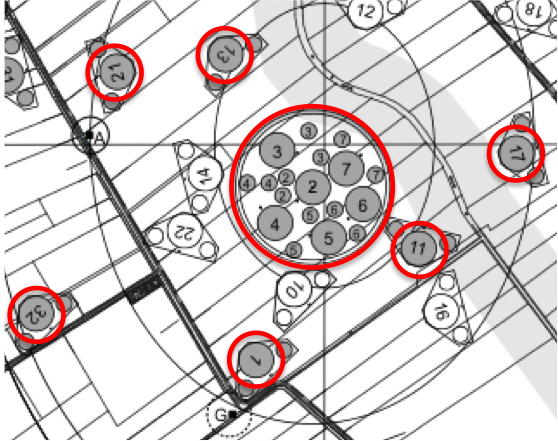
\includegraphics[width=1\textwidth]{Figs/afaac12_arrayconfig.png}
\caption{The spatial distribution of AARTFAAC-12 stations within the core of LOFAR stations.}
\label{fig:afaac12_arrayconfig}
\end{figure*}

Figure \ref{fig:afaac12_arrayconfig} shows  the LOFAR stations that  are part of
the AARTFAAC system.

\begin{figure*}[htbp]
\centering
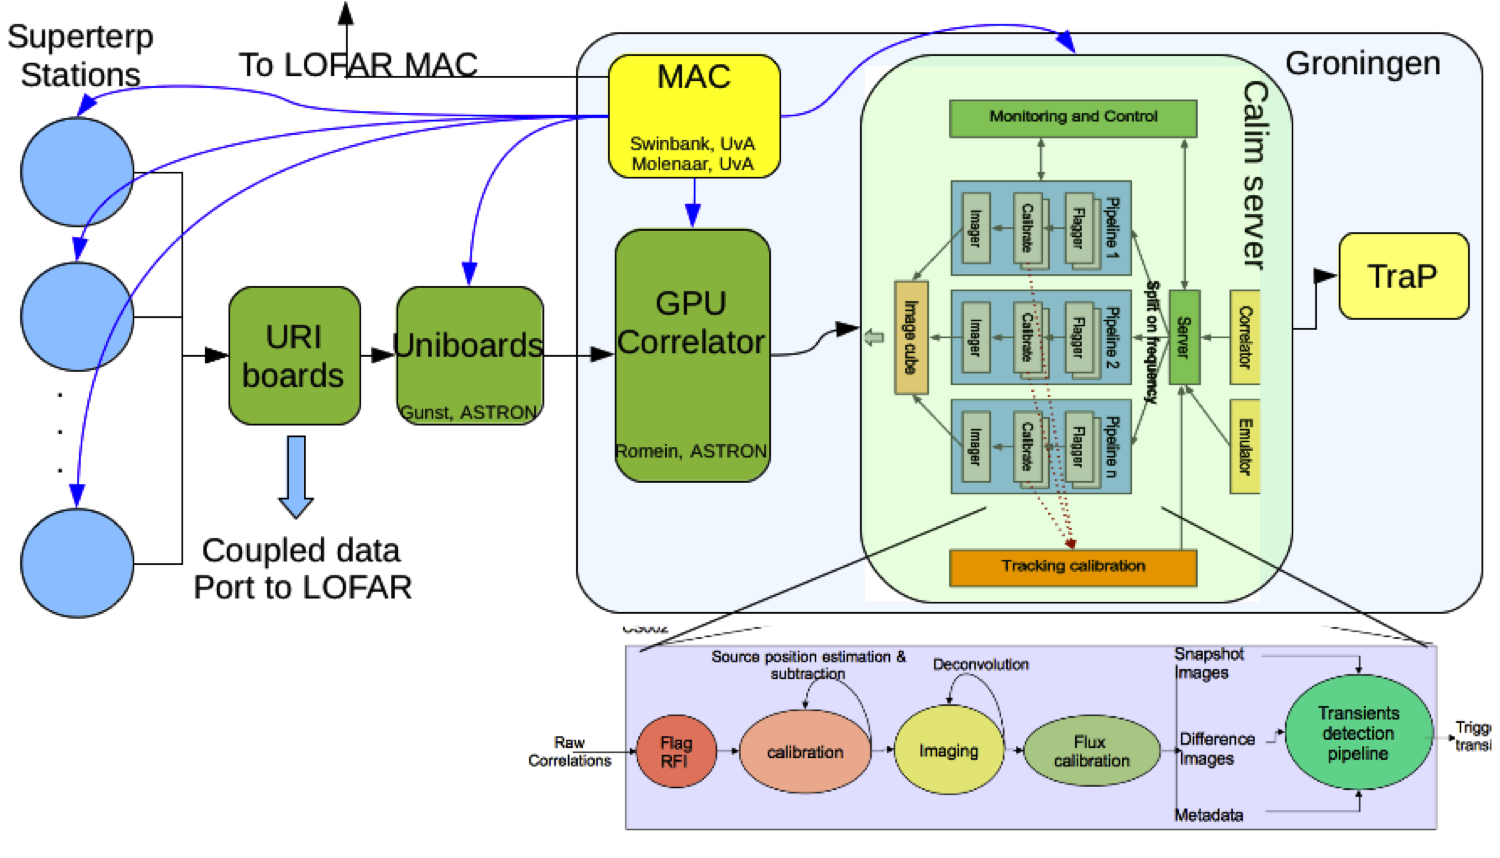
\includegraphics[width=1\textwidth]{Figs/overall_afaac_Arch_blks.png}
\caption{Overall architecture of the AARTFAAC all-sky monitor depicting each processing subblock.}
\label{fig:afaac_arch}
\end{figure*}

The overall  architecture of  the radio  sky monitor  is shown  schematically in
Figure \ref{fig:afaac_arch},  and illustrates  the main processing  subblocks of
the  instrument. A  user  selectable subset  of subbands  from  every dipole  is
transferred  as UDP  packets over  a dedicated  10Gbit fiber  connection to  the
central  processing  systems.  These  are   received  by  a  streaming  software
correlator  implementation  which aligns  the  data  and estimates  the  spatial
covariance matrix between every pair of dipoles.  The generated visibilities are
streamed  over TCP/IP  to a  calibration  and imaging  pipeline component  which
carries out autonomous imaging.  The images are then analyzed by a software tool
(The  Transients Pipeline,  TraP), which  extracts the  light curves  of sources
within  the  image,  and  analyses  them  for  variability  using  a  number  of
parameters. The TraP is described in more detail in \ref{}.

The specifications of the AARTFAAC monitor are listed in Table TODO.

TODO: For  Eric.
\textbf {Remote Station Processing:} The above  processing is carried out in the
Remote Station Processor  (RSP), an FPGA board which can  handle the beamforming
of TODO: X subbands for 4 dipoles. The further stages of beamforming are carried
out  by distributing  the 4-dipole  beamformed data  over a  station level  ring
network.

\textbf {Available bit modes:} 

\textbf {Ring network sharing for dipole level data products:}

\begin{figure*}[htbp]
\centering
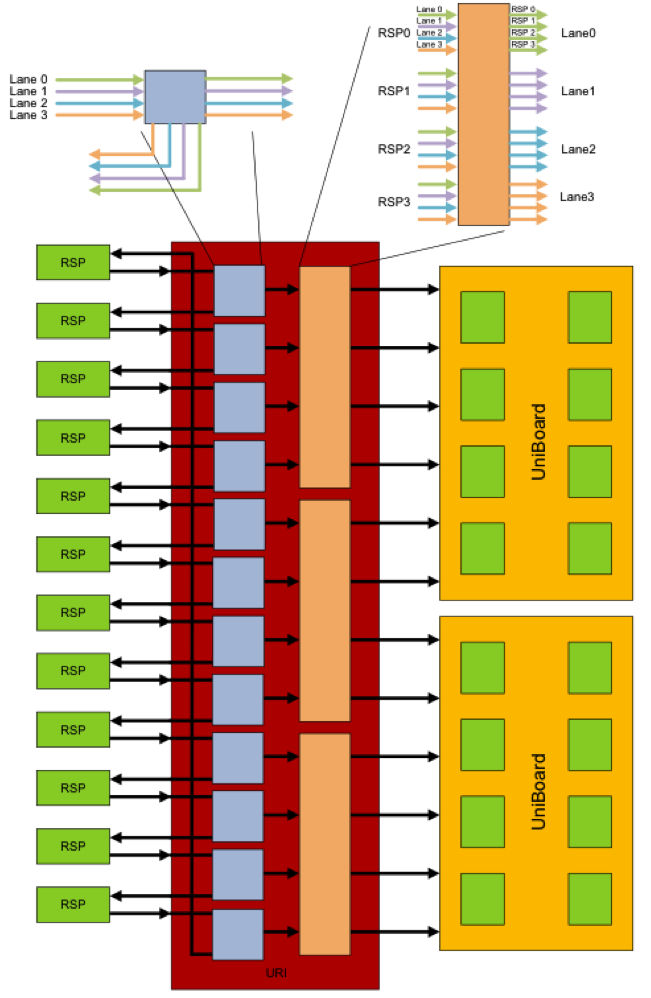
\includegraphics[width=1\textwidth]{Figs/station_hw_proc_afaac.png}
\caption{The station level hardware changes  allowing creation of a coupled data
  path for AARTFAAC data flow.}
\label{fig:afaac_station_hw}
\end{figure*}

Figure \ref{fig:afaac_station_hw} depicts the  station level ring network, whose
bandwidth is shared between the beamformed  subbands as well as the dipole level
subbands. The ring network bandwidth constrains the processed AARTFAAC bandwidth
to a fundamental maximum of 64 4-bit subbands, or about 12MHz. The URI boards in
combination with  the uniboards  carry out  a first level  of the  incoming data
transposition.


\subsection {\label{subsec:impact_lofar} Impact of sharing dipoles with LOFAR on AARTFAAC}
LOFAR operates using either  the LBA or the HBA antenna at  a time. Further, due
to limited station level electronics for stations within the core, only a subset
of the available station dipoles can be utilized. This implies that the AARTFAAC
telescope  is  dependent  on  LOFAR  for  the  choice  of  antenna  and  station
configuration,  reducing the  availability  for all-sky  monitoring. Within  the
station, only the LBA\_OUTER station  configuration is currently deemded suitable
for  real-time imaging.   This mode  of  LOFAR operation  favorable to  AARTFAAC
depends on  the observing  schedule and the  proposed observations.   Table TODO
shows some  statistics from previous cycles  on the fraction of  observing modes
favorable to AARTFAAC. Based on this, it  may be resonable to expect AARTFAAC to
operate TODO fraction of time, typically.

\section {\label{sec:station_hardware} Station level hardware for piggy-back operation}
\begin {itemize}
 \item {URI board  description, data coupling scheme,  constraints on achievable
   bandwidth}
 \item  {The uniboard  data  reformatting (transpose),  uniboard data  transfer,
   output data format}
 \item {Available diagnostics, performance, commissioning tests}
\end{itemize}

\section {\label{sec:gpucorr} The AARTFAAC real-time correlator}
\begin{figure*}[htbp]
\centering
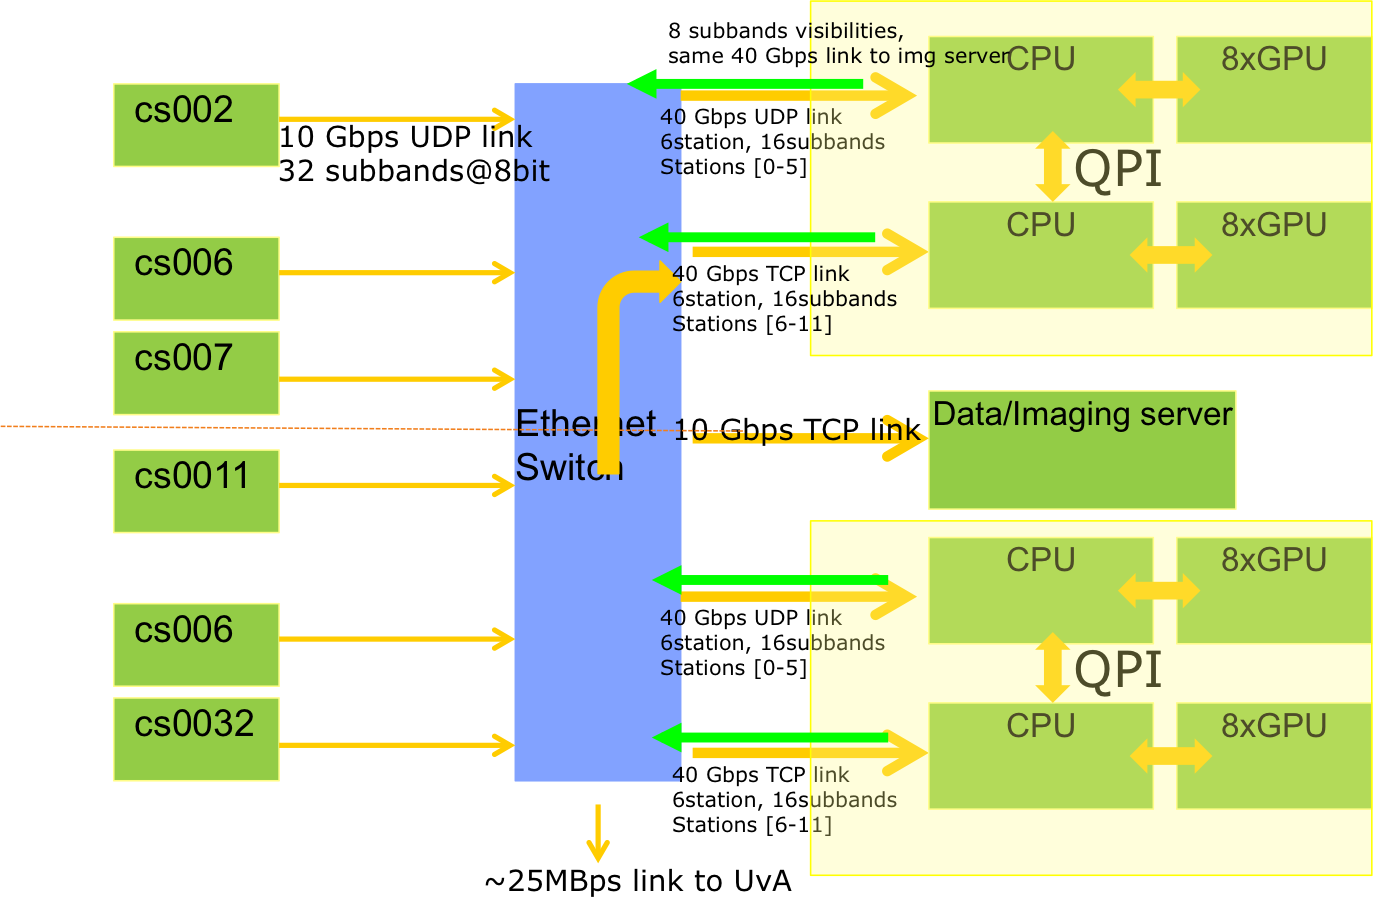
\includegraphics[width=1\textwidth]{Figs/correlator_arch.png}
\caption{The GPU correlator implementation using a pair of AMD(?) CPUs hosting AMD GPUs}
\label{fig:afaac_station_hw}
\end{figure*}

\begin {itemize}
 \item {Correlation for transit mode observations: logical blocks.}
 \item {Description of processing flow.} 
 \item {Motivation of chosen architecture for implementation.}
 \item {Supported time and frequency binning, motivation of choice.}
 \item {Required compute and memory bandwidth.}
 \item {Synchronization of incoming data (input buffer), output data format.}
 \item {Commissioning tests, performance.}
\end {itemize}

\section {\label{sec:calim} Real-time calibration and imaging}
\begin {itemize}
 \item {Architecture, implementation choices, performance}
 \item {Unit test architecture}
 \item {Interface to TraP}
\end {itemize}

\section {\label{sec:acontrol} The AARTFAAC control interface}
\begin{figure*}[htbp]
\centering
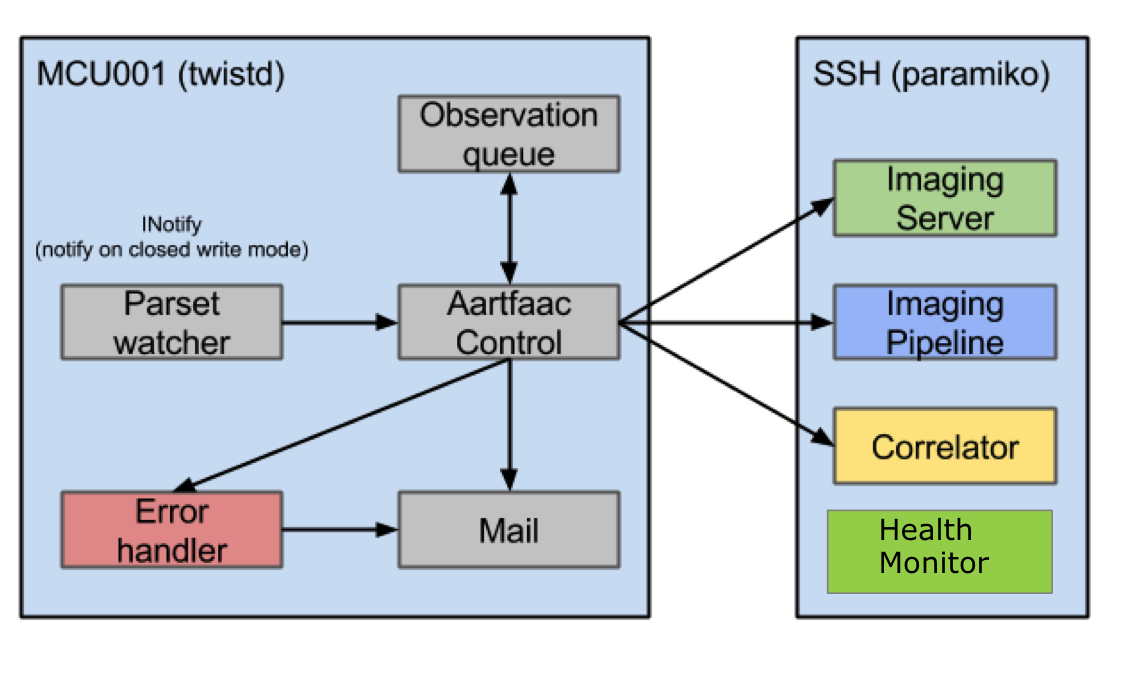
\includegraphics[width=1\textwidth]{Figs/control_sys.png}
\caption{The  control  system  architecture  which  interfaces  with  the  LOFAR
  observation scheduling system and triggers AARTFAAC observations.}
\label{fig:afaac_ctrl_sys}
\end{figure*}
Figure  \ref{fig:afaac_ctrl_sys} shows  the  functional blocks  of the  AARTFAAC
control system, and their interface to the LOFAR scheduling system.
\begin {itemize}
 \item {Control system description}
 \item {Interface with LOFAR}
 \item {Monitoring interface: AARTFAAC webpage}
\end {itemize}

\section {\label{sec:results} Commissioning results}
\begin {itemize}
 \item {Long term performance of the entire system based on logs.}
 \item {Performance  in various  bit-modes, with  different number  of subbands,
   expected sensitivity.}
\end {itemize}

\section {\label{sec:discussion} Discussion}

\section {\label{sec:conclusion} Conclusions}

\begin {acknowledgements}

This work  was funded  by the ERC  grant <num> awarded  to Prof.   Ralph Wijers,
Universitiet  Van Amsterdam.   We  thank The  Netherlands  Foundation for  Radio
Astronomy  (ASTRON)  for support  provided  in  carrying out  the  commissioning
observations.
\end{acknowledgements}
\bibliographystyle{aa}
\bibliography{ref}

\end{document}
